\documentclass[11pt,a4paper,parskip]{scrartcl}
%\def\xcolorversion{2.00}
%\def\xkeyvalversion{1.8}
\usepackage[utf8x]{inputenc}
%\usepackage{ucs}
\usepackage{amsmath}
\usepackage{amsfonts}
\usepackage{amssymb}
\usepackage{graphicx}
\usepackage{lmodern}
\usepackage{hyperref}
\usepackage[ngerman]{babel}
\usepackage{pdfpages}
%\usepackage[version=0.96]{pgf}
\usepackage{tikz} %Tikz
\usepackage{pgfplots}
\usepackage[acronym, toc]{glossaries} %Glossar
\makeglossaries
\newglossaryentry{Ablaufberg}{
    name=Ablaufberg,
    description={Der Ablaufberg ist ein in der Regel künstlich angelegter Hügel, über den ein Gleis verläuft. Ablaufberge dienen beim Abdrücken dem Ablaufen lassen von Güter- wagen, die auf diese Weise nach ihren Bestimmungsorten sortiert werden}
}
%	Bedienfahrt	
%	Bezetteln   
\newglossaryentry{Bremsprobe}{
    name=Bremsprobe,
    description={Eine Bremsprobe  ist ein zur Vorbereitung von Zugfahrten gehörender Vorgang, bei dem die Funktionsfähigkeit des Bremssystems der Fahrzeuge im Zugverband überprüft wird. Dabei wird im Stillstand das Anlegen und Lösen der zu prüfenden Bremsen kontrolliert%. Siehe dazu auch Anhang \ref{sec:ABremsen}
    }
}
\newglossaryentry{Eisenbahnverkehrsunternehmen}{
    name=Eisenbahnverkehrsunternehmen,
    description={Eisenbahnverkehrsunternehmen sind Eisenbahnen, die Eisenbahnverkehrsleistungen erbringen. \acrshort{EVU}s müssen in der Lage sein, die Zugförderung (Traktion) sicherzustellen\cite{rennsteigbahn}}
}
\newglossaryentry{Heisslaeuferortungsanlage}{
    name=Hei\ss l\" auferortungsanlage,
    description={Eine Heißläuferortungsanlage dient dazu, eine unzulässige Er- wärmung von Radsatzlagern durch Defekte bei Schienenfahrzeugen (sogenannte Heiß- läufer) rechtzeitig feststellen zu können}
}
\newglossaryentry{ep-Bremse}{
    name=ep-Bremse,
    description={Die elektropneumatische Bremse (ep-Bremse) ist eine durch elektropneumatische Bauteile gesteuerte automatische Druckluftbremse bei Eisenbahnen. Die ep-Bremse ermöglicht das gleichzeitige Bremsen oder Lösen aller Fahrzeuge unabhängig von der Länge des Zuges}
}
\newglossaryentry{ep-''light''-Bremse}{
    name=ep-''light''-Bremse,
    description={Was genau macht sie jetzt?
    }
}
\newglossaryentry{EOW}{
    name=EOW,
    description={Eine elektrisch ortsgestellte Weiche (EOW) ist eine elektrisch angetriebene Weiche, die nicht von einem Stellwerk, sondern vom Weichenort aus direkt bedient wird. EOW sind das moderne Äquivalent zu Handweichen und werden hauptsächlich in Gleisanlagen eingesetzt, in denen nur frei rangiert wird}
}
\newglossaryentry{Bergbremse}{
    name=Bergbremse,
    description={Bergbremsen sorgen bei großen Rangierbahnhöfen nach erfolgter Geschwindigkeitsmessung für eine Vorabbremsung, damit die Talbremsen ihre Funktion erfüllen können}
    }
\newglossaryentry{Talbremse}{
    name=Talbremse,
    description={Talbremsen verzögern Wagen vor einer Richtungsgleisgruppe, so dass der Abstand zum vorherlaufenden Wagen groß genug bleibt, damit die Weichen in der Lücke umgestellt werden können}
    }
\newglossaryentry{Gleisanschluss}{
    name=Gleisanschluss,
    description={Ein Gleisanschluss ist ein Schienenweg zur Erschließung eines Geländes oder Gebäudes, das selbst nicht zur öffentlichen Eisenbahninfrastruktur gehört}
}
\newglossaryentry{Hemmschuh}{
    name=Hemmschuh,
    description={Ein Hemmschuh ist eine keilförmige Konstruktion zum Festhalten von Schienenfahrzeugen. Er wird zwischen Rad und Schiene platziert, um durch die entstehende Reibung den Wagen zu bremsen beziehungswies an (selbstständiger) Bewegung zu hindern}
}
\newglossaryentry{Knotenbahnhof}{
    name=Knotenbahnhof,
    description={Ein Knotenbahnhof ist eine Bahnhof der für Betriebsabläufe zur Zugbereitstellung oder Verknüpfung mit anderen Verkehrsträgern erforderlich ist}
}
\newglossaryentry{Rangierbahnhof}{
    name=Rangierbahnhof,
    description={Rangierbahnhöfe sind die Zugbildungsbahnhöfe des Einzelwagenverkehrs im Güterverkehr der Eisenbahn}
}
\newglossaryentry{Rangierfahrt}{
    name=Rangierfahrt,
    description={Rangierfahrten bezeichnen das Bewegen einzelner Schienenfahrzeuge oder Fahrzeuggruppen, soweit es sich nicht um eine Zugfahrt (einschließlich Sperrfahrt) handelt}
}
%\newglossaryentry{Rangiermittel}{
 %   name=Rangiermittel,
  %  description={Rangiermittel sind Ein- oder Zweiwegefahrzeuge die (mit Elektroantrieb und oder im Handbetrieb) Die Aufgaben von Rangierlokomotiven übernehmen.}
%}
\newglossaryentry{Satellitenbahnhof}{
    name=Satellitenbahnhof,
    description={Satellitenbahnhöfe bestehen in der Regel aus kleinen Gleisanlagen ohne Rangiereinrichtungen und -personal. Sie dienen der Sammlung und Verteilung Güterwagen auf die Lokalen Gleisanschlüsse\cite{Verkehrslogistik}}
}
%\newglossaryentry{Sägefahrten}{
 %   name=Sägefahrten,
  %  description={Sägefahrten sind das koordinierte Vor- und Zurücksetzen von Wagen zum rangieren von Wagen.}
%}
\newglossaryentry{Schiebewandwagen}{
    name=Schiebewandwagen,
    description={Der gedeckte Güterwagen der Sonderbauart H, oder auch Schiebewandwagen, ist ein gebräuchlicher Wagen für nässeempfindliche, pallettierte Ware. Die verschieblichen Seitenwände ermöglichen es, die ganze Ladefläche von der Seite her zu be- und entladen}
}
\newglossaryentry{Sperrfahrt}{
    name=Sperrfahrt,
    description={Sperrfahrten sind Fahrten, die in ein Gleis der freien Strecke eingelassen werden, das gesperrt ist. Dies dient der Bedienung einer Anschlussstelle auf der freien Strecke\cite{RIL408}}
}
\newglossaryentry{Zugfahrt}{
    name=Zugfahrt,
    description={Eine Zugfahrt bezeichnet eine Fahrt im Bahnhof und auf der Strecke, die durch Hauptsignale gesichert und geregelt ist, sowie Züge im Bereich mit Führerstandsignali- sierung. Bei dieser Fahrt ist der Fahrweg bis zum Ende frei. Es wird Flankenschutz gewährt und Weichen gegen Umstellen gesichert. Die Strecke für die Zugfahrt hat eine maximale Geschwindigkeit vorgegeben, der Zug hat eine feste Zusammensetzung und eine eindeutige Zugnummer für diese Fahrt}
}
\newglossaryentry{Zugschluss}{
    name=Zugschluss,
    description={	Der Zugschluss bezeichnet den letzten Wagen eines Zuges. Dieser ist vom Zugschlusssignal gekennzeichent. Mit seiner Hilfe kann die Vollständigkeit von Zügen, visuell durch das Personal des Bahnbetriebs, überprüft werden}
}
\newglossaryentry{Vorbahnhof}{
    name=Vorbahnhof,
    description={Als Vorbahnhof bezeichnet man den äußeren Teil eines großen Bahnhofes oder auch einen Bahnhof in der Nähe eines großen Bahnhofs, der diesem Aufgaben abnimmt}
}
\newglossaryentry{Lokrangierfuehrer}{
    name=Lokrangierf\"uhrer,
    description={Der Lokrangierführer ist eine Bezeichnung für einen Triebfahrzeug- führer oder einen Eisenbahnfahrzeugführer von Lokomotiven mit Funkfernsteuerung im Rangierdienst}
}
\newglossaryentry{Eisenbahnbetriebsleiter}{
    name=Eisenbahnbetriebsleiter,
    description={Eisenbahnbetriebsleiter leiten und überwachen die sicherheitsrelevanten Abläufe in einem Eisenbahnunternehmen, das keinen grenzüberschreitenden Verkehr aufweist}
}
\newglossaryentry{Bremsprobeberechtigte}{
    name=Bremsprobeberechtigte,
    description={Der Bremsprobeberechtigte ist ein für die Bremsprobe ausgebildeter Mitarbeiter, der die Bremsprobe durchführen darf. Häufig haben Triebfahrtzeugführer diese Zusatzausbildung selbst, um die Bremsprobe selbstständig durchführen zu können}
}
\newglossaryentry{Bremsprobeanlage}{
    name=Bremsprobeanlage,
    description={Eine Bremsprobeanlage wird für die Herstellung der Betriebsbereitschaft eines Eisenbahnzuges benötigt. Sie dient dazu eine Hauptbremsprobe am Zugverband durchzuführen. Diese Hauptbremsprobe kann zwar auch ohne eine entsprechende (ortsfeste) Anlage durchgeführt werden, dann muss aber ein Triebfahrzeug und ein weiterer Bremsprobeberechntigter vorhanden sein. Aus Kostengründen werden deshalb in größeren Formationsbahnhöfen ortsfeste Bremsprobeanlagen eingesetzt, da damit Triebfahrzeuge und Personal eingespart werden können}
}

\newglossaryentry{konventioneller Gueterwagen}{
    name=konventioneller G\"uterwagen,
    description={Als konventionelle Güterwagen werden die Güterwagen bezeichnet, die aus konventionellen (herkömmlichen) Komponenten, wie Drehgestellen, Kupplungen, Bremsen und Wagenkästen, bestehen}
}

\newglossaryentry{Gueterwagen 40}{
    name=G\"uterwagen 4.0,
    description={Als Güterwagen 4.0 wird der vollständig ausgebaute Güterwagen bezeichnet}
}

\newglossaryentry{Demonstrator}{
    name=Demonstrator,
    description={Als Demonstrator wird der in diesem Projekt modifizierte Güterwagen bezeichnet. Er stellt eine Teilmenge des Güterwagen 4.0 dar}
}

\newglossaryentry{40-Komponenten}{
    name=4.0-Komponenten,
    description={4.0-Komponenten sind die Subsysteme, die den konventionellen Güter- wagen zu einem Güterwagen 4.0 machen. Zu diesen Komponenten gehören die Energieversorgung, Aktoren und Sensoren sowie die Kommunikationssysteme des Güterwagen}
}

\newglossaryentry{Wagenzug}{
    name=Wagenzug,
    description={Ein Wagenzug ist ein gekuppelter Verband nicht angetriebenen Güterwagen}
}

\newglossaryentry{Zugverband}{
    name=Zugverband,
    description={Ein Verbund aus Güterwagen und Lok wird als Zugverband bezeichnet}
}

\newglossaryentry{Lastwechsel}{
    name=Lastwechsel,
    description={Die Ausstattung mit Lastwechsel ermöglicht das Anpassen des Bremsklotzdrucks an das effektive Wagengewicht. Sie verhindert ein Überbremsen bei geringer Zuladung und wirkt zu schwacher Bremskraft bei beladenen Fahrzeugen entgegen. Wenn bei gleichbleibender Bremskraft das Fahrzeuggewicht durch die Beladung zunimmt, verringert sich die Bremswirkung. Darum ist die Umstelleinrichtung in die passende Stellung („leer“, „beladen“ oder ggf. „teilbeladen“) manuell oder automatisch zu bringen}
}
%\newacronym{AK}{AK}{Automatikkuppung}
\newacronym{DIN}{DIN}{Deutsches Institut für Normung}
%\newacronym{EOW}{EOW}{Elektisch ortsgestellte Weiche}
\newacronym{EN}{EN}{Europäische Normung}
\newacronym{EVU}{EVU}{Eisenbahnverkehrsunternehmen}
%\newacronym{FHAC}{FH Aachen}{Fachhochschule Aachen, University of applied Science}
\newacronym{HL}{HL}{Hauptluftleitung}
%\newacronym{ISO}{ISO}{International Organisation for Standardisation	(dt.: Internationale Organisation für Normung)}
\newacronym{RIL}{RIL}{Richtlinie}
\newacronym{twb}{TWb}{Technische Wagenbehandlung}
\usepackage{verbatim}
%Quellen Beginn
    \usepackage[backend=bibtex,
        style=numeric,
        bibencoding=ascii
        %style=alphabetic
        %style=reading
    ]{biblatex}
    \addbibresource{Kapitel/Quellen.bib}
%Quellen Ende
%Anforderungsnummerierung nach Raphael Beginn
    %\theoremstyle{remark}
    \newtheorem{rem}{Notiz}
    %\theoremstyle{definition}
    \newtheorem{feat}{Merkmal}
    %\newtheoremstyle{definition}% name of the style to be used
    %  {5pt}% measure of space to leave above the theorem. E.g.: 3pt
    %  {5pt}% measure of space to leave below the theorem. E.g.: 3pt
    %  {}% name of font to use in the body of the theorem
    %  {}% measure of space to indent
    %  {\bfseries}% name of head font
    %  {}% punctuation between head and body
    %  {\newline}% space after theorem head; " " = normal interword space
    %  {}% Manually specify head
%Anforderungsnummerierung nach Raphael Ende


\begin{document}

\setlength{\parskip}{5mm}% plus5mm minus5mm} %Absatzlänge
%Deckblatt Beginn
\begin{titlepage}
    \newcommand{\HRule}{\rule{\linewidth}{0.5mm}} % Defines a new command for the horizontal lines, change thickness here
    \center % Center everything on the page
    \vspace*{2cm}
    \textsc{\LARGE Neue Elektronik- und Kommunikationssysteme für den intelligenten, vernetzten Güterwagen}\\[1.5cm] % Name of your university/college
%    \textsc{\Large Neue Elektronik- und Kommunikationssysteme für den intelligenten, vernetzten Güterwagen}\\[0.5cm] % Major heading such as course name
    \textsc{\large FKZ 16ES0850K}\\[0.5cm] % Minor heading such as course title
    \HRule \\[0.4cm]
    { \huge \bfseries Lastenheft}\\[0.4cm] % Title of your document
    \HRule \\[1.5cm]
    \begin{minipage}{0.4\textwidth}
    \begin{flushleft} \large
    \emph{FH Aachen}\\
    Daniela \textsc{Wilbring}\\
    Prof. Dr.-Ing. Manfred \textsc{Enning},\\
    Prof. Dr.-Ing. Bernd \textsc{Schmidt},\\
    Prof. Dr. Raphael \textsc{Pfaff}\\
    \end{flushleft}
    \end{minipage}
    ~
    \begin{minipage}{0.4\textwidth}
    \begin{flushright} \large
    \end{flushright}
    \end{minipage}\\[2cm]
    {\large \today}\\[2cm] % Date, change the \today to a set date if you want to be precise
    \vfill % Fill the rest of the page with whitespace
\end{titlepage}
%Deckblattt Ende
\section*{Zweck des Dokuments}
Das Lastenheft ist, nach DIN 69901-5\footnote{Projektmanagement – Projektmanagementsysteme – Teil 5: Begriffe}, ''die vom Auftraggeber festgelegte Gesamtheit der Forderungen an die Lieferungen und Leistungen eines Auftragnehmers innerhalb eines (Projekt-)Auftrags''.\par
Ein Lastenheft ist wichtig in der Analysephase und zur Kommunikation innerhalb des Auftrages/Projekts. Es bietet eine ausführliche Beschreibung der Arbeitsleistung und dient als Kommunikationsbasis.\par
Auf Basis des Lastenheftes wird das Pflichtenheft vom Auftragnehmer erarbeitet.\par
Untersuchungen zeigen, dass Fehler in der Produktentwicklung bei einer späten Aufdeckung und Behebung teurer werden als bei einer früheren Erkennung. Deshalb sollte man schon beim Lastenheft eine hohe Qualität anstreben.\footnote{Quelle: \url{https://www.pm-blog.eu/themen/methoden/lastenhefte-eine-schrittweise-anleitung-fur-den-perfekten-aufbau.html} }\par
In diesem Fall wird das Lastenheft im Rahmen des Projektes "Neue Elektronik- und Kommunikationssysteme für den intelligenten, vernetzten Güterwagen" von der FH Aachen als Vorarbeit für das Pflichtenheft erstellt. \par
Klare gemeinsame Ziele innerhalb des Projektes sollen zu einer besseren und strukturierten Zusammenarbeit führen.
%Das Lastenheft wird aufgrund von Veröffentlichungen der Projektsteller und dem Gesamtverbundantrag des Projektes erstellt


\section*{Revisionshistorie}
\begin{tabular}{|p{3cm}|p{2cm}|p{5.5cm}|p{2cm}|}
\hline
Versionsnummer  & Datum         & Beschreibung          & Autor     \\
\hline
 1.0.0          & 28.02.2019    & Erstellung Lastenheft & Wilbring  \\\hline
                &               &                       &           \\\hline
\end{tabular}

% Aufbau Versionsnummmer
% 1.2.3
    % 1 - Hauptversionsnummer - Signifikante Änderung am Lastenheft - Änderungnen Inhaltsverzeichnis, Strukturänderung, ...
    % 2 - Nebenversionsnummer - Funktionale Änderung am Lastenheft - weitere Anforderungen, Ausführungen in Unterkapiteln, ...
    % 3 - Revisionsnummer - Kleine Änderungen am Lastenheft - Fehlerbehebung, Orthographie, ...\newpage
\tableofcontents \newpage
%\printglossary[title= Abkürzungen, toctitle=Abkürzungen, type=\acronymtype]
%\printglossary\newpage
%\section{Einleitung}
Der Güterverkehr in Deutschland wird bislang zu über 70\% von LKWs gestemmt, was Verkehrsstaus und hohe Schadstoffemissionen verursacht. Das Zukunftsprojekt Industrie 4.0 bietet dem Schienengüterverkehr die einzigartige Chance, durch intelligente Steuerung und Vernetzung Transportprozesse extrem flexibel, effizient und schadstoffarm zu gestalten. Realisiert werden kann dies durch die Integration vielfältiger moderner Sensorik und Elektronik in den Güterwagen4.0.\footnote{Antrag auf Gewährung einer Bundeszuwendung auf Ausgabenbasis (AZAP), 26.04.2018}\par
%Im Projekt werden Sensoren und Elektroniksysteme zur Realisierung eines „intelligenten“, mittels Industrie 4.0-Technologien vernetzten Güterwagens entwickelt. Die Sensorik dient dabei der Online-Erfassung relevanter Güterwagen- und Zugverbund-Daten zur Zustands- und Verschleißanalyse. Durch diese Informationen wird erstmals eine durchgängige Logistik und die von Kunden geforderte Transparenz der Lieferkette sowie eine vorausschauende Planung von Wartungszyklen und Rentabilität für den Güterwagenbetreiber ermöglicht. Als weiterer Lösungsansatz werden Aktoren entwickelt und in den Güterwagen4.0 integriert, mit denen die beim Zusammenstellen bzw. Trennen von Güterwagen erforderlichen aufwendigen und oft sicherheitsrelevanten manuellen Tätigkeiten künftig vollautomatisiert durchgeführt und sensorisch online überwacht werden können.\footnote{Antrag auf Gewährung einer Bundeszuwendung auf Ausgabenbasis (AZAP), 26.04.2018}\\
%Der Güterwagen4.0 stellt einen wichtigen Baustein zur Lösung der gravierenden Verkehrsprobleme dar. Die Ergebnisse des Vorhabens tragen wesentlich dazu bei, durch einen zukunftsfähigen Schienenverkehr Verkehrsstaus und Schadstoffemissionen zu vermindern. Die angestrebten sensorischen Fähigkeiten des Güterwagen4.0 erlauben perspektivisch auch eine Übertragung in den Schienenpersonenverkehr.\footnote{Antrag auf Gewährung einer Bundeszuwendung auf Ausgabenbasis (AZAP), 26.04.2018}\\\\
In diesem Lastenheft wird anhand eines Schiebewandwagens der grobe Ablauf eines Umlaufs im bisherigen System erläutert und daraufhin Anforderungen an den neuen Güterwagen erstellt. Als Motivation zeigen sich %neben der oben bereits erwähnten Verringerung von Verkehrsstaus und Schadstoffemissionen auch 
eine Erhöhung der Prozesssicherheit, Verringerung der aufzuwendenden Zeit am Wagen, eine Gestaltung von attraktiveren Arbeitsplätzen durch eine ergonomischere Arbeitsgestaltung und mögliche Kosteneinsparungen an der Infrastruktur.\par
Herausforderungen wie die Migration und Annahme des Systems sollen beachtet werden. Die Kosten des Systems, sowie dessen Einbau müssen konkretisiert werden. Prozesse für produktivere Arbeitsabläufe mit dem neuen Güterwagen müssen gestaltet werden. Arbeitsabläufe bei Defekten konkretisiert werden.\\

Hier fehlt eine Erklärung wo die Reise hin gehen soll, ein Fokus, was wir uns vom GW40 erhoffen und eine sensibilisierung für den Prozess und das Vorgehen zur Änderung dessen.\\
Es ist geplant eine Möglichkeit für produktivere Verkehre zu schaffen.\\
Automatisierungslösungenen  Automatisches Abdrücken mit AK o. automatischer Schraubenkupplung – Trennstellen, Kommunikation mit Bergrechner – Vorbereitung Ablauf\\
• Vorteile des Systems\\
Dezentralität\\
Zukunftssicher\\
muss nicht auf AK warten, funktioniert aber auch damit\\
Wertschöpfungsprozess\\
Automatisierung\\
Automatisierung Bremse – Bremse lösen, lüften, Handbremse, Berechnung Bremsgewichte, Durchgängigkeit HL, automatische Bremsprobe, automatischer Bremszettel\\
Vorbereitung Trennstellen – HL-Absperrhähne Schließen, lüften, 2x Signal = trennen – Signal: kann, soll trennen %\newpage
\section{Ist-Zustand}\label{sec:Istzustand} %Beschreibung wo Produktivität vergudet wird um daraus ableiten zu können, was benötigt wird. % Kochsiek, Knoll nach Meinung zu diesem Kapitel fragen!
Im Folgenden wir der Umlauf eines \gls{Schiebewandwagen} (Habinns) beschrieben. Der Wagen wird in einem \gls{Gleisanschluss}/RailPort mit palletiertem Gut beladen, läuft dann durch das deutsche/europäische Einzelwagensystem und wird in einer Ladestelle an einem Gleisanschluss oder RailPort entladen. Fokus dieser Beschreibung sind die durchzuführenden manuellen Tätigkeiten. Davon leitet sich im Folgenden ein Anforderungskatalog an einen aktiven, kommunikativen Güterwagen 4.0 ab, der viele oder alle der manuellen Tätigkeiten durch Technikfunktionen ersetzt.
Die hier beschriebenen Prozesse sind leicht idealisiert. So werden Störfälle erst einmal ausgenommen. Auch kann davon ausgegangen werden, dass jede Prozess leicht anders aussieht. Trotzdem zeigt er viele wichtige Punkte, die verbessert werden können und sollten. Bei anderen Wagenarten unterscheidet sich der Umlauf natürlich noch weiter. Weitere Informationen zu anderen Prozessen und vor allem auch zu Prozessen in der Disposition sind im Anhang \ref{sec:realeIst} zu finden. \par
\subsection{Vorgänge an der Ladestelle/im Gleisanschluss}
%In diesem Unterkapitel wird eine kurze Beschreibung def Fahrwege, Bewegung von Fahrzeugen, der Personaltätigkeit sowie der Beladung, dem Wagenwechsel, der Ladungsicherung und der benötigten Transportdokumente gegeben.
\subsubsection{Fahrweg} \label{sec:Fahrweg}
Die Bewegung von Wagen erfolgt prinzipiell auf Gleisen. Eine Verzweigung von Fahrwegen erfordert Weichen. In kleinen und mittleren Gleisanschlüssen sind dies überwiegend handbetätigte Weichen. 
\subsubsection{Bewegung der Wagen} \label{sec:BewdWagen}
Je nach Wagenaufkommen kommen folgende Methoden der Wagenbewegung in Betracht:
\begin{itemize}
	\item Bedienung durch das \acrshort{EVU}, welches auch die Zustellfahrten durchführt
	\item Eigene (zum \gls{Gleisanschluss} zugehörige) Rangierlokomotive
	\item Eigenes Rangierhilfsmittel
	\begin{itemize}
	    \item Gleisfahrbar (Rangierroboter)
	    \item Zweiwegefahrzeug
	\end{itemize}
	\item Stationäre Verschubeinrichtung (Seilzuganlage)
	\item Verschub mittels Muskelkraft von Tieren oder Menschen (z.B. Knippstange, Wagenrücker)
\end{itemize}
\subsubsection{Personalfähigkeiten}\label{sec:Personal}
Allen Methoden ist gemeinsam, dass Sie spezielle Personalfähigkeiten bzw. eine entsprechende Ausbildung benötigen. Dies ist nicht zuletzt auf die Tatsache zurückzuführen, dass ein einmal in Bewegung gesetzter Güterwagen auch bei langsamer Fahrt eine hohe kinetische Energie aufweist. Zusätzlich ist die Bedienung der Wagenbremsen (Luft- und/oder Handbremse) für ungeschultes Personal kompliziert und fehleranfällig.
\subsubsection{Bereitstellung}
Eine Bereitstellung der Wagen findet aus einem \gls{Vorbahnhof} als Einfahrgruppe oder Ordnungsgruppe statt. Diese stehen dort im Allgemeinen mit entlüfteter Bremse und vorgelegtem Hemmschuh oder angelegter Handbremse.
\subsubsection{Beladung}
Das Beladen von Güterwagen mit Paletten erfolgt von einer Rampe oder einer Ladekante mit Überfahrbrücke aus in der Regel per Gabelstapler. Im Gegensatz zur Heckbeladung von LKW existieren kaum Lösungen zur Automatisierung der Beladung. Dies ist ein Logistikprozess des Verladers.
\subsubsection{Ladungssicherung}
Während oder nach der Beladung muss die Ladung gegen Verrutschen gesichert werden. Bei Schiebewandwagen erfolgt dies unter anderem durch von Hand verschiebbare und durch Verriegeln zu sichernde Zwischenwände. Auch für diese Aufgabe ist der Verlader verantwortlich. Er muss den Wagen als bahntechnisch sicher an das EVU übergeben. Das EVU darf nur mit einem augenscheinlich (also für den Beobachter sicheren) Wagen fahren. Dies betrifft in einem geschlossenen Wagen nicht die Ladung, aber die Türen und Verschlüsse; auf einem offenen (Holz-)Transporter aber auch die sichtbare Ladung. Bei Gefahrgut müssen noch weitere Kontrollen von geschultem Personal durchgeführt und der Wagen passend gekennzeichnet werden.
\subsubsection{Wagenwechsel}
Eine Ladekante ist meist für Einzelwagen oder kleine Gruppen (bis max. ca. 4 Wagen) gestaltet, so dass häufig Wagen an der Ladestelle getauscht werden müssen, bevor die Zustellfahrt erfolgt. Dies liegt unteranderem an der Seitenbeladung, für die viel Platz benötigt wird. Diese hat, gegenüber der Heckbeladung bei LKW, den Vorteil der Parallelisierbarkeit. LKW gehen nach der Beladung direkt in den Umlauf, sodass bei diesen das häufige Umsetzen nicht als Nachteil gesehen wird. \par
Beim Beladen von Wagen mit Gefahrgut, ist es üblich die Weichen vor und hinter der Beladestelle in der dem Beladegleis abgewandten Position abzuschließen. Dies soll ein ungewolltes Bewegen der Wagen verhindern. Diese Weichen werden vom Verlader erst nach Beenden der Verladearbeiten wieder geöffnet.\par
Wagen können grundsätzlich rangiert oder verschoben werden. Findet die Wagenbewegung mit \gls{Lokrangierfuehrer} (\acrshort{LRF}) und Lok statt, wird rangiert. Verschoben werden die Wagen wenn die Wagenbewegung ohne Lok und Lokrangierführer stattfindet.\par
Rangiert wird wenn möglich ohne Luftkupplung und entsprechend auch ohne \gls{Bremsprobe}. Ob Rangieren ohne Luftkupplung möglich ist, hängt von der Lokomotive, der Last, der Achsenanzahl der zu rangierenden Wagen und der Neigung des Ladegleises ab. Muss aufgrund dieser Eigenschaften mit Luft gefahren werden, ist auch eine vereinfachte \gls{Bremsprobe} notwendig. Häufig findet diese Rangierfahrt in der Bremsstellung G statt.\par
Im Allgemeinen werden einzelene Wagen oder kleinere Wagengruppen für nur wenige Meter verschoben. Dies kann zum Beispiel mit einem Zwei-Wege-Fahrzeug auf LKW-Basis stattfinden. Hier verschiebt ein angelernter und unterwiesener Verlademitarbeiter mit einem zusätzlichen Sicherheitsposten die Wagen. Der Verlademitarbeiter wird vom \gls{Eisenbahnbetriebsleiter} (\acrshort{EBL}) angelernt und unterwiesen.
\subsubsection{Transportdokumente}\label{sec:Transdoc}
Im LKW-Bereich entstehen bereits Lösungen zur papierlosen Transportabwicklung einschließlich der Behandlung von Gefahrgutdokumenten. Bei Bahntransporten herrscht die klassische Methode der Übergabe von Frachtdokumenten an das \acrshort{EVU} vor. Oft werden diese auch direkt elektronisch übergeben. Dann sind diese später digital verfügbar. Ausgenommen sind Gefahrgutscheine, diese werden immer als Papierzettel mitgeführt. Auch die Wagen werden, vorallem im Einzelwagenverkehr noch "`bezettelt"'\footnote{Siehe dazu auch VDV-Schrift 758 - Prüfen von Güterwagen im Eisenbahnbetrieb}. Diese Zettel sind Vereinfachungen des Frachtbriefes, die direkt auf dem Wagen mitgeführt werden. Auf diesen steht im Allgemeinen aus was die Ladung besteht, woher diese kommt und wohin sie geht. Auch weitere Besonderheiten werden hier vermerkt.
%Der Lkw wird meist in Längsrichtung durch das Heck an einem Tor / Vorsatzschleuse beladen. Für die eigentliche Beladung ist es  ungünstiger als die Seitenbeladung, es führt aber zu einer effizienten Flächennutzung in der Halle (Zeilenstruktur). Daher ist die Heckbeladung gerade bei Logistik/Verteilzentren und Speditionen heute die vorherrschende Methode.  
%Für spezielle Güter / Wagen ist Beladung mit Hallenkran von oben üblich (Papier, Stahlcoils)
\subsection{Abholen im Gleisanschluss}
Die Abholung von Wagen erfolgt entweder durch das \acrshort{EVU} unmittelbar an der Ladestelle oder -- wenn lokale Rangierhilfsmittel zur Verfügung stehen -- von einem Übergabegleis im Werksgelände. Die Bedienung des Anschlusses ist in der Regel Teil eines Umlaufs, in dem mehrere Anschlüsse nacheinander bedient werden.
\subsubsection{Luft- und mechanische Kupplung}\label{sec:LuftumechKup}
Der oder die Wagen stehen im festgelegten Zustand zur Abholung bereit. Die Luftbremse ist gewöhnlich außer Funktion, der Reserveluftbehälter ist leer. Nach dem Ansetzen der Lok bzw. des aktuell letzten Wagens der Rangierabteilung ist manuell zu kuppeln. Der Lokführer oder Rangierbegleiter "`taucht"' dazu unter den Puffern durch und verbindet zunächst manuell die Schraubenkupplung. Danach wird die Hauptluftleitung gekuppelt und die Absperrhähne der \acrshort{HL} geöffnet. %prüfen
\subsubsection{(Vereinfachte) Bremsprobe}\label{sec:vBremsprobe}
Im Anschluss erfolgt eine (vereinfachte) \gls{Bremsprobe}. Dazu wird zunächst am letzten Wagen der Gelöstzustand überprüft, dann der \acrshort{HL}-Druck abgesenkt und das Führerbremsventil abgesperrt. Die Bremsen müssen anlegen. Im Anschluss wird zur Durchgängigkeitsprüfung wieder die Fahrstellung eingenommen und das \acrshort{HL} Absperrventil des letzten Wagen für mindestens 15 Sekunden geöffnet. Die Bremsen müssen anlegen und wieder lösen.
\subsubsection{Technische Wagenbehandlung}\label{sec:tWb}
Vor Beginn der Rangier-/\gls{Sperrfahrt} ist eine technische Wagenbehandlung (\acrshort{twb}) der Stufe 1 (siehe dazu auch Anhang \ref{sec:ATWb}) durchzuführen. 
\subsubsection{Zustellfahrt}\label{sec:Zustellfahrt}
Erfolgt die Zustellfahrt über die freie Strecke, ist das Streckengleis durch das Stellwerk für \gls{Zugfahrt}en zu sperren. Wenn der Gleisanschluss selbst nicht als Bahnhof ausgebildet ist, also keine eigenen Ausfahrsignale besitzt, erfolgt die Fahrt als \gls{Sperrfahrt}. Wenn der \gls{Gleisanschluss} an ein Bahnhofsgleis angeschlossen ist, handelt es sich um eine \gls{Rangierfahrt}. In jedem Fall ist es eine Fahrt auf Sicht mit geringer Geschwindigkeit. Worst Case für die Nutzung der Strecke mit \gls{Zugfahrt}en wäre eine geschobene \gls{Sperrfahrt}, diese ist nicht nur mit geringer Geschwindigkeit sondern auch mit höherem Personalaufwand durch Besetzung der Spitze verbunden.

\subsection{Fahrt zum Knotenbahnhof und Zugbildung}
\subsubsection{Zugfahrt zum Satellitenbahnhof}\label{sec:Zugfahrt}
Satellitenbahnhöfe sind Bahnhöfe, in dem im Einzelwagenverkehr \gls{Zugfahrt}en enden oder beginnen. Sie sind in der Regel für die Übergabegruppe nur Durchgangsstation. Die Kombination der Übergabe mit weiteren Übergaben von anderen Anschlüssen/Satelliten erfolgt im \gls{Knotenbahnhof}. Weil die Fahrt vom Satelliten- zum \gls{Knotenbahnhof} eine \gls{Zugfahrt} (mit in der Regel Geschwindigkeiten $\ge 80 km/h$) darstellt, ist vor Beginn der Fahrt eine Berechnung des Bremsgewichts und eine volle \gls{Bremsprobe} durchzuführen.%erfragen
\subsubsection{Rangiervorgänge im Umsetzbetrieb}\label{sec:Rangierfahrt}
Knotenbahnhöfe können über \gls{Ablaufberg}e verfügen. In der Regel ist dies aber nicht der Fall und die Rangiervorgänge finden im so genannten Umsetzbetrieb statt. Dabei werden jeweils Wagengruppen angekuppelt (je nach Lok ist die Kupplung der Luft meist nicht notwendig) und durch eine Sägefahrt in ein anderes Gleis versetzt und dort gekuppelt. Das Stellen der Weichen für diese Vorgänge erfolgt meist vom Stellwerk des Bahnhofs aus oder durch eine \gls{EOW}\footnote{Elektrisch ortsgestellte Weichen}-Anlage.
\subsubsection{Übergabe der Wagen}\label{sec:UEdWagen}
Wie bei der Abholung aus dem Gleis muss auch vor der Abfahrt des aus Übergaben zusammengestellten Zuges eine \gls{Bremsprobe} und eine technische Wagenbehandlung durchgeführt werden. Außerdem sind erneut Bremsgewicht und Bremshunderstel zu berechnen. Bei jeder Zugzusammenstellung sind Papiere zu prüfen und zu übergeben.

\subsection{Fahrt zum Knotenbahnhof des Zielbereichs über einen oder mehrere Rangierbahnhöfe}
\subsubsection{Rangiervorgänge im Knotenbahnhof}\label{sec:RangKnoten}
Ab dem \gls{Knotenbahnhof} sind die weiteren Fahrten/Umstellvorgänge wie folgt charakterisiert:
\begin{itemize}
    \item Züge haben idealerweise die volle Länge von 700 m
    \item Zugumstellungen erfolgen in den großen Rangierbahnhöfen
\end{itemize}
Wie bei einem Postverteilsystem haben die Rangierbahnhöfe die Aufgabe, hereinkommende Züge aufzulösen und die Wagen auf neue Züge umzustellen, die sie ihrem Ziel näher bringen. Dieser Abschnitt des Einzelwagenverkehrs ist hochautomatisiert und -produktiv. Dennoch verbleiben auch hier große Automatisierungslücken. 
\subsubsection{Vorprüfung}\label{sec:Vorpruefung}
Am Beispiel der Behandlung der Wagen in einem automatisierten \gls{Rangierbahnhof} wird dies deutlich:\par
Nach der Einfahrt des Zuges in die Einfahrgruppe wird durch den so genannten "`Vergleicher"' die Übereinstimmung der übermittelten Zugliste mit der tatsächlichen Reihung geprüft. Grund für diesen scheinbar überflüssigen Schritt ist die Tatsache, dass das Herausrangieren von fehlerhaften Wagen auf der Strecke (meist in der Folge einer Alarmmeldung einer Heißläuferortungsanlage) nicht in der Informationstechnik berücksichtigt wird.\par
Die weiteren Schritte bei der Vorbereitung sind wie folgt:
\begin{enumerate}
    \item Zugbremse anlegen, \acrshort{HL} entlüften, Lok abkuppeln
    \item Zug festlegen (i.d.R. durch \gls{Hemmschuh}e)
    \item Wagen/-gruppen vereinzeln. Dafür an den vorgesehenen Trennstellen nach Zerlegeliste Luft- und mechanische Schraubenkupplungen trennen und Luftbremse durch Ziehen am Lösezug lösen (Entlüften der A-Kammer/des Reserveluftbehälters). Je nach Rangierverfahren wird die Schraubenkupplung komplett ausgehängt (vorentkuppelt abdrücken) oder sie wird lose eingehängt gelassen und erst am \gls{Ablaufberg} durch den "`Stangler"' ausgeworfen.
\end{enumerate}
\subsubsection{Abdrücken am Ablaufberg}\label{sec:Abdruecken}
Wenn in Kapitel \ref{sec:Vorpruefung} beschriebenen Vorbereitungen abgeschlossen sind, wird der Zug zum Abdrücken freigegeben. Die Abdrücklokomotive schiebt dann -- nach dem Entfernen der Hemmschuhe -- den Zug mit Geschwindigkeiten von 1,2 bis 3 m/s %ist das so?
über den \gls{Ablaufberg}. Hinter dem Gipfel vereinzeln sich die Wagen. Durch den Schwerkrafteinfluss, werden diese durch ein gestaffeltes System von mechanischen Gleisbremsen, auf die Eintrittsgeschwindigkeit im Richtungsgleis heruntergebremst und laufen langsam in die Richtungsgleise ein.  Klassisch ist dies das Arbeitsfeld der Hemmschuhleger, die durch gezieltes Platzieren von Hemmschuhen die Wagen punktgenau vor dem letzten Wagen im Richtungsgleis abbremsen.
\subsubsection{Automatisiertes Abdrücken}\label{sec:automAbdruecken}
In den großen Rangierbahnhöfen sind die Fortschritte der Automatisierungstechnik sichtbar. In allen Anlagen gibt es automatische Steuerungen der Verteilweichen. In einigen Anlagen sind die Ablaufsteuerungen mit einer automatischen Steuerung der Abdrücklokomotiven gekoppelt, so das während des Abdrückvorgangs kein manueller Steuer- eingriff notwendig ist; Die Rückfahrt der Lok zum nächsten Einsatz bleibt aber Handarbeit.In allen Anlagen werden die Bremsen (Bergbremse und Talbremse) geregelt betrieben, so dass unterschiedliche Laufeigenschaften der Wagen und Windeinflüsse automatisch kompensiert werden und in den meisten Anlagen ist das Legen von Hemmschuhen zur Zielbremsung ersetzt worden durch automatische Fördereinrichtungen, die so genannten Räum- und Beidrückförderer.\par
Wenn dieser hochautomatisierte Prozess für den betrachteten Wagen im Richtungsgleis abgeschlossen ist, geht es wieder in Handarbeit weiter.
\subsubsection{Zugvorbereitung}\label{sec:Zugvorbereitung}
Nach dem Schließen des Richtungsgleises für weitere Abläufe werden die Wagen provisorisch miteinander gekuppelt und die Wagengruppe wird in ein Gleis für die Nachbehandlung gezogen. In einigen Anlagen erfolgt die Nachbehandlung im Richtungsgleis. Dort werden die folgenden Schritte durchgeführt:
\begin{enumerate}
    \item Mechanisch kuppeln
    \item Luftleitungen kuppeln, \acrshort{HL} Absperrhähne öffnen
    \item \acrshort{HL} Absperrhahn am (neuen) \gls{Zugschluss} schließen, Zugschlusstafel stecken
    \item Bremsberechnung (Zuggewicht, Bremsgewicht, Bremseigenschaften der Lok)
    \item Bremsstellungswechsel je nach Bremsart der folgenden \gls{Zugfahrt}
    \item Volle \gls{Bremsprobe}, in der Regel mittels stationärer \gls{Bremsprobeanlage}
    \item Technische Wagenbehandlung, Stufe 3
\end{enumerate}
\subsubsection{Nachordnung}
Falls die örtlichen Verhältnisse in den Zielgleisanschlüssen und die Reihenfolge von deren Bedienung bekannt sind, erfolgt noch eine Nachordnung der Wagen nach Empfängern durch einen erneuten Berglauf oder in einer Nachordungsgruppe. Dieses ist effizienter als manuelle Umstellvorgänge mittels Sägefahrten in Knoten oder Satellitenbahnhöfen.

\subsection{Fahrt zum Satellitenbahnhof}
\subsubsection{Zugfahrt}
Der im Knotenbahnhof vorbereitete Zug wird dann für den nächsten Abschnitt von der vorgesehenen Streckenlok übernommen. Nach einer vereinfachten \gls{Bremsprobe} kann die \gls{Zugfahrt} beginnen.\par
\subsubsection{Umsetzbetrieb}
Am Satellitenbahnhof angekommen wird der Zug wieder, wie oben beschrieben, im Umsetzbetrieb umgestellt. Dabei werden
jeweils Wagengruppen angekuppelt (je nach Lok ist die Kupplung der Luft meist nicht notwendig) und durch eine Sägefahrt in ein anderes Gleis versetzt und dort gekuppelt.
\subsubsection{Übergabe der Wagen/Zugvorbereitung}
Auch  vor  dieser  Abfahrt  wird der  zusammengestellte  Zug wieder mittels \gls{Bremsprobe} und technischer Wagenbehandlung geprüft, ebenso die dazugehörigen Papiere.

\subsection{Fahrt zum Gleisanschluss/zur Ladestelle}
Wenn die Zustellfahrt über die freie Strecke erfolgt, ist das Streckengleis für Zugfahrten zu sperren. Diese Fahrt kann als Sperrfahrt oder Rangierfahrt stattfinden.
\subsubsection{Rausrangieren einzelner Wagen}
Angekommen am \gls{Gleisanschluss} müssen einzelne Wagen wieder aus dem Zugverband rausgangiert oder zumindest abgekuppelt werden.
\subsubsection{Entladen}
Angekommen am \gls{Gleisanschluss} muss der Wagen noch zur Entladestelle gebracht werden und entladen werden. %\newpage
\section{Soll-Zustand}
In diesem Kapitel sollen einzelne Themen aus dem Ist-Zustand herausgegriffen und mittels für das Projekt ausgebautem Güterwagen 4.0 beschrieben werden.\par
Hier werden vorstellbare Punkte ausgeführt, die aber nicht alle zur Standardausrüstung gehören müssen oder sollten. Eine einfache Nachrüstung soll möglich sein.\par
Durch eine Energieversorung als Basis des Güterwagens 4.0 ist es möglich verschiedene Seonsorik des Wagens speisen sowie die Kommunikation zwischen einzelnen Güterwagen sowie einem Server und verschiedenen mobilen Endgeräten herstellen, aber auch eine sporadische Aktorik für die Bremse ermöglichen. Die Punkte werden einzeln anhand von Aufgaben aus der Ist-Beschreibung beschrieben. \par
Durch diese Erweiterung des konventionellen Güterwagens soll der Güterwagen ein besseres Arbeitsmittel auf dem Werksgelände und in Zugbildungsanlagen werden.
\subsection{Allgemeines}
Es wird der Sollzustand des Demonstrators beschrieben und nicht des späteren vollständig ausgebauten Güterwagen 4.0.\par
Die Aufbauten auf dem Demonstrator sollen vor Zugfahrten vollständig abschaltbar sein.
\subsection{Energieversorgung}
Dieses Kapitel beschreibt die Energieversorgung des Güterwagens 4.0 für dieses Projekt. Es beschreibt weder die Energieversorgung des späteren 'vollständig' ausgebauten Güterwagen 4.0  noch die Energieversorgung der VDI-Richtlinie 5905. Dabei wird es wahrscheinlich Überschneidungen geben, auch werden Erfahrungen aus den Arbeitsrunden mitgenommen und einfließen, aber es wird keine exemplarische Realisierung dessen.\par
Aufgrund der Prototypenentwicklung in diesem Projekt erscheint eine 24 V-Spannungs- versorgung für dieses Projekt sinnvoll. Sowohl werden alle Grenzen der Berührspannungen im Kleinspannungsbereich eingehalten, als auch gibt es bereits sehr viele Produkte auf dieser Spannungsebene. Namentlich genannt die SPS, aber auch diverse Sensoren und Aktoren.\par
Gepuffert werden soll das System durch eine Batterie. Diese Batterie soll genügend Leistung liefern um sämtliche Daten-, Kommunikations- und Aktorsteuerungesprozesse speisen zu können. Außerdem soll sie genug Energie für den Erprobungsbetrieb bieten. Sie soll mittels Ladegerät nachladbar sein, aber auch eine Schnittstelle für einen Achsdeckelgenerator haben. Zum Aufladen wird dieser wahrscheinlich nicht geeignet sein, da keine entsprechenden Umlaufzyklen während der Testphase möglich sind. Diese sollen aber während des Projektes simuliert werden.\par
Eine Ausstattung als Nachrüstung von konventionellen Güterwagen muss in der Konstruktion bedacht werden. Eine Beladung des Güterwagens und im restlichen Umlauf soll im Projektverlauf simuliert werden.\par
Für die Versorgung von Sensoren und Aktoren ist für dieses Projekt ein Klemmkasten vorzusehen, der in zukünftigen Projekten professionalisiert werden kann. Die Batterie ist in einem Einschubkasten so anzubringen, dass sie von außen zugänglich ist, aber auch vor Steinschlag und ähnlichem während einer Fahrt geschützt ist. Die Verrohrung für Daten- und Stromleitungen ist vorzusehen, sodass diese geschützt sind und klare Linien zur Verlegung von Leitungen zu sehen sind. Ein Anschluss im Anschlusskasten anzusetzen. Für die Batterie ist eine Ladeschnittstelle von 230 V anzusetzen. Sämtliche Anbauten sollen unter ATEX-gerechten Bedingungen angebracht werden, das bedeutet unter anderem, dass keine zur Explosion neigenden Materialien verwendet werden dürfen, kein Gasaustausch stattfindet und alles bahnrobust ausgelegt ist.\par
\subsection{Verhalten an der Ladestelle}

Verladung von Paletten:
Sensoren für alle Komponenten der Ladungssicherung
Technische Überwachtung von verschiedenen Sensoren/Hebeln (DK) Ladungssicherung - Railbuisness S. 3 > Näherungsschalter und Stellhebel -- königszapfen
automobilverladung --Ladeverstellung
Containertragwagen -- Tragzapfen
Coiltransporter
Schiebewandwagen - verstellbare und verschließbare Trennwände
Spanngurt mit Sensoren in Textilien?

Sensoren können Probleme bei Funkkommunikation machen -- Kabel besser? Diskussion
Vorstellbar auch temperatursensoren - Licht um den Güterwagen zur Warnung, Alarmanlage
\subsection{Wagenbewegungen}
Wagenbewegung mittels Rangierhilfsmittel 
mit und ohne Luft
Regel: Festgebremst, wenn keine Luft, lose, wenn Luft. + manuelle Einstellung
Handbremse leicht bedienbar. Beispielsweise über Device, oder "Knopfdruck" am Wagen
Stillstandsüberwachung - Warnlichter - Rundumlicht (Hat auf Werksgelände sonst alles (ist das so? Joachim fragen) oder/und Akustik
Warnfunktion an der Spitze beim Rangieren + Kamera für Unimogfahrer? Fahrer eines Zwei-Wege-Fahrzeuges auf LKW-Basis
Automatische Notbremsfunktion - Handbremse anlegen bei Hindernis - Vorstellbar, aber Standardausrüstung? Wirtschaftliche Betrachtung
\subsection{Wagenzusammenstellung}
TWb und Bremsprobe
BP: Wagen soll Bremsfähigkeit angeben und erproben, eine Rückmeldung geben, Druck im Reservebehälter anzeigen über Sensorik, HL/C-Druck für Bremsprobe, Wie viel Druck brauche ich außer Druck auf dem Bremszylinder?
Bremseinstellung / Lastwechsel vornehmen - Abgeschaltete Bremse melden
Alle Sensoren prüfen - Bereitschaft und Wert iO - und rückmeldung geben
Beispiele: Dreh-(Kugel)Pfanne am Drehgestell (VTG), Bremsbelag überwachung, Lagerzustände (während der Fahrt), erste Meter: Lagerschaden, Flachstelle, Entgleisungssicherheit (vRang = 25 km/h)
HL-Absperrventile immer automatisch in richtiger Position: REgel: Wagen dran = offen, Wagen ende = zu

Mit anderen Sprechen wegen automatischer BRemsprobe
\subsection{Zugfahrt}
Volle Bremsprobe
LL Einstellbar

\subsection{Datenhaltung und -übertragung}
Daten im Wagen über separates Kabel, zum nächsten Wagen nur kurze Funkstrecken
Es soll eine Kommunikation relaisiert werden. Sowohl zw. Sensoren und Rechner, Wagen, Wagen und Wagen - Device
Bedienung erfordert Datentechnische Verbindung. Auch zu Device in der ok
Reichweite? ausreichend, nicht von außen störbar, nicht abhörbar
Bandbreite? ausreichend
Zugriffsmöglichkeiten auf Daten nach Authorisierung. Verschiedene Authorisierungsstufen und Geofencing.
\subsection{Diagnosefunktionen}
vorausschauende Wartung
alles über sich wissen, was er wissen muss und speichern und abrufbar machen

\subsection{Wagen als Bestandteil im IT-Güterverkehr}
Wagen als Bestandteil im IT-Güterverkehr
elektronischer Ladezettel
Betriebsinfos lokal auf Wagen
Wartungsinfos in der Cloud %\newpage
\section{Anforderungsbeschreibung}
\textbf{Einfügen: Wie lang sind Lösezeiten, Verwendung Handbremse, Umlegen Endabsperrhähne}\par
Zielgrupper - Rangierende, WagenmeisterInnen, Bremsprobeberechtige, Tf, ...\par
\textbf{Sicherheitsrelevanz, Bedienen, Beobachten, Anbringungspunkte von Bauteilen -- gefedert? -- Bahntauglichkeit}\par
\begin{figure}[htbp] 
    	\begin{center}
            		\begin{tikzpicture}[scale = 1]
		\draw[line width = .6cm, gray!30, -stealth] (-1.5,6.3) -- (-1.5,0);
                                \begin{axis}[ 
                                font = \small,
                                width = 10cm, height = 8cm,
                                xbar, xmin=0, xmax = 55,
                                xlabel={Zeit [min]},
                                symbolic y coords={%
                                {Freigabe prüfen},{Bremse freigeben},{Bremsung prüfen}, {Bremsen betätigen}, {Dichtigkeitsprüfung}, {Zustandsbewertung},{Füllen Bremsleitung},{Zugvorbereitung} },
                                ytick=data,
                                nodes near coords, 
                                %nodes near coords align={horizontal},
                                ytick=data,
                                % nodes near coords align={vertical},
                                bar width=7pt,
                %            legend style={
                   %             at={(1,1.1)},
                    %      	anchor=east},
                  %              legend columns = 2,
                                ]
                                \addplot coordinates {                          
                                (39.5,{Zugvorbereitung})
                                (40,{Füllen Bremsleitung})
                                (33.2,{Zustandsbewertung})
                                (1,{Dichtigkeitsprüfung})
                                (1,{Bremsen betätigen})
                                (33.2,{Bremsung prüfen})
                                (2,{Bremse freigeben})
                                (33.2,{Freigabe prüfen})
%                                (183.1,{Sum})
                                };
                                %\addlegendentry{Wagon $<$ 4.0}
                                \addplot coordinates {                          
                                (1,{Zugvorbereitung})
                                (10,{Füllen Bremsleitung})
                                (1,{Zustandsbewertung})
                                (1,{Dichtigkeitsprüfung})
                                (1,{Bremsen betätigen})
                                (1,{Bremsung prüfen})
                                (2,{Bremse freigeben})
                                (1,{Freigabe prüfen})
%                                (18,Sum)
                                };
                                %\addlegendentry{Wagon 4.0}
                                \end{axis}
                              \end{tikzpicture}
        		\end{center}
    \caption{Zeitvergleich Bremsprobe und automatisierte Bremsprobe nach \cite{Stephenson}}
    \label{fig:Zeitvergleich}
\end{figure} 
Abbildung \ref{fig:Zeitvergleich} zeigt einen Zeitvergleich zwischen konventioneller Bremsprobe (blau) und automatisierter Bremsprobe (rot). Hier sieht man vor allem, dass  bei Zugvorbereitung, Füllen der Bremsleitung, Zustandsbewertung der Wagen und Überprüfung ob die Bremsen angelegt und wieder gelöst haben viel Zeit eingespart werden kann. Dies ist in den vorigen Kapiteln beschrieben.\par
Anhand des Ist- und Soll-Zustandes sind fünf Ausbaustufen für den Güterwagen 4.0 geplant, die diese Zeiteinsparung bringen sollen. Hier eine Kurzbeschreibung der geplanten Ausbaustufen:\par
\textbf{Ausbaustufe 1: Stromversorgung, Telematik und Datenvernetzung}\par
\begin{figure}[hbp] 
    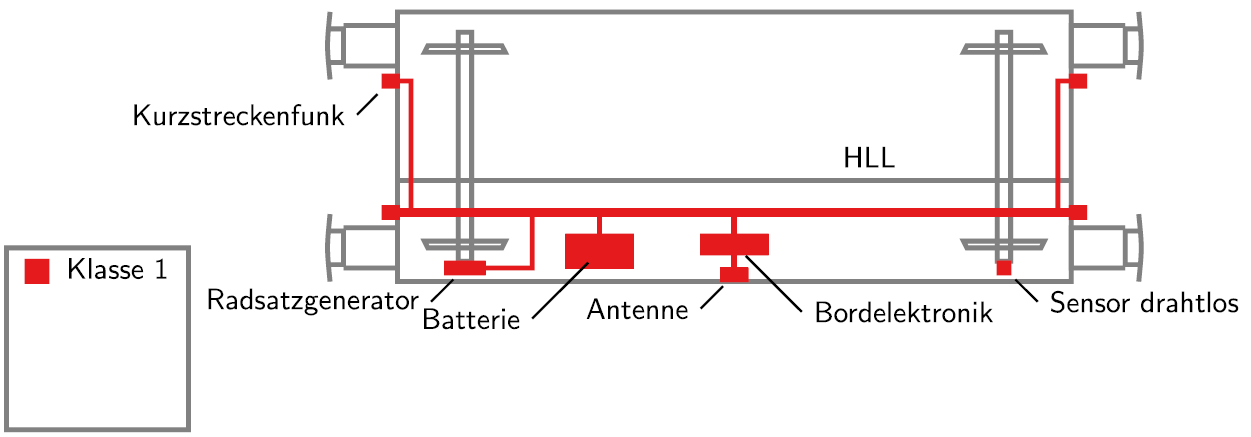
\includegraphics[width=\textwidth]{Bilder/Ausbaustufen_1.PNG}
    \caption{Klasse 1 mit Stromversorgung, Telematik und Datenvernetzung - angelehnt an \cite{Ausbaustufen} }
    \label{fig:Klasse1}
\end{figure} 
In der ersten Ausbaustufe, siehe Abbildung \ref{fig:Klasse1}, ist geplant Bordelektronik und eine entsprechende Spannungsversorgung anzubringen. Diese kann als Batterie mit Speisung durch einen Radsatzgenerator, Solarpanels oder ähnlichem realisiert werden oder auch als Pufferbatterie mit Speisung durch AK. Dazu kommen verschiedene Antennen und Kurzstreckenfunk zur Kommunikation mit anderen Wagen. Auch Sensoren zur Erfassung verschiedener Telematikfunktionen sind geplant.\par
In diesem Stadium ist der Wagen an sich noch nicht 'schlauer' als ein nicht ausgerüsteter Wagen, aber er kann sich mitteilen. Mitteilungen könne sein: Standort, Belandung, Laufleistung, (ungewöhnliche) Vibrationen (beispielsweise durch Falschstellen), Heißläuferdedektion, letzte Wartungsintervalle, Zustand der Bremse und vieles mehr.\par
\textbf{Ausbaustufe 2: Ausbaustufe 1 + Automatisierung der Bremsbedienung}\par
\begin{figure}[htbp] 
    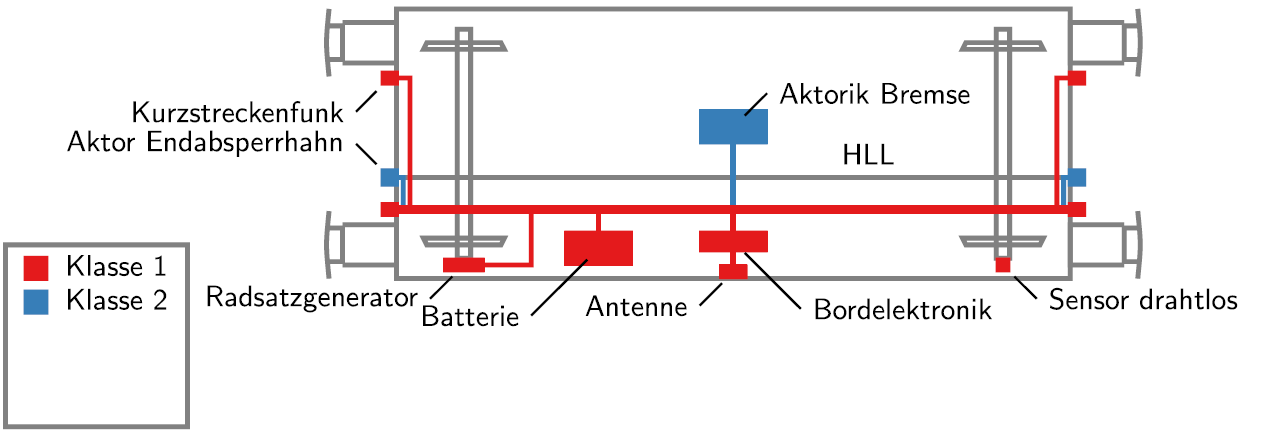
\includegraphics[width=\textwidth]{Bilder/Ausbaustufen_2.PNG}
    \caption{Klasse 2 bestehend aus Klasse 1 und der Automatisierung der Bremsbedienung - angelehnt an \cite{Ausbaustufen}}
    \label{fig:Klasse2}
\end{figure} 
In der zweiten Ausbaustufe ist eine zusätzliche Aktorik für Endabsperrhähne und Handbremse geplant. Dadurch kann ein Teil der Bremsbedienung sow weit automatisiert werden, dass ein Einstellen der Bremsart anhand von anderen Wagen im Wagenzug, Gewicht und Bremsfähigkeit möglich ist. Außerdem ist die automatische Parkbremse realisiert.\par
\textbf{Ausbaustufe 3: Ausbaustufe 2 + ep-''light''-Bremsen}\par
\begin{figure}[htbp] 
    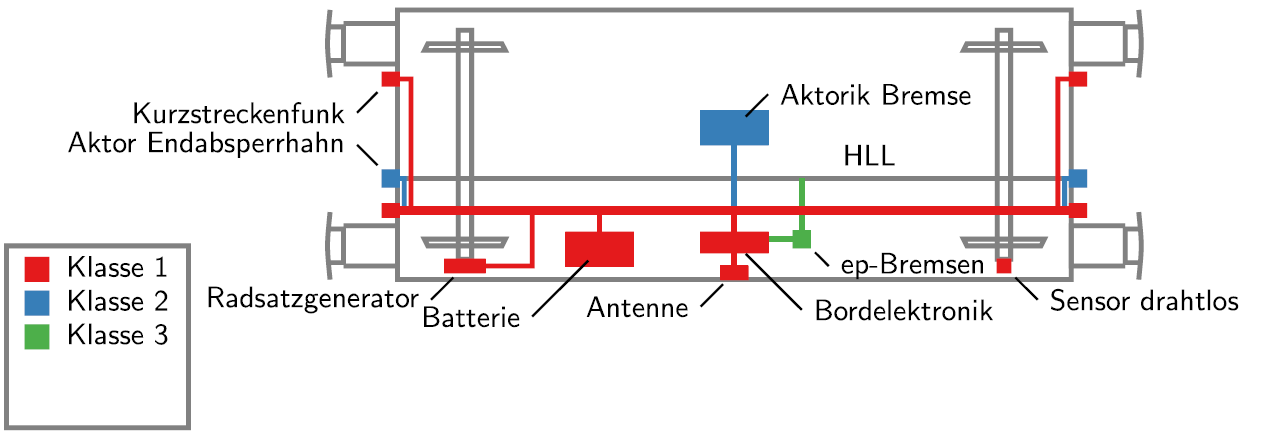
\includegraphics[width=\textwidth]{Bilder/Ausbaustufen_3.PNG}
    \caption{Klasse 3 bestehend aus Klasse 2 und der eingeführten ep-''light'-Bremse - angelehnt an \cite{Ausbaustufen}}
    \label{fig:Klasse3}
\end{figure} 
In der dritten Ausbaustufe kommt zusätzlich zur Bremsbedienung auch die Ep-''light''-Bremse hinzu. Diese sorgt für eine für kürzere Bremswege und/oder höhere Geschwindigkeiten.\par
\textbf{Ausbaustufe 4: Ausbaustufe 3 + automatisierter Zugschluss}\par
\begin{figure}[htbp] 
    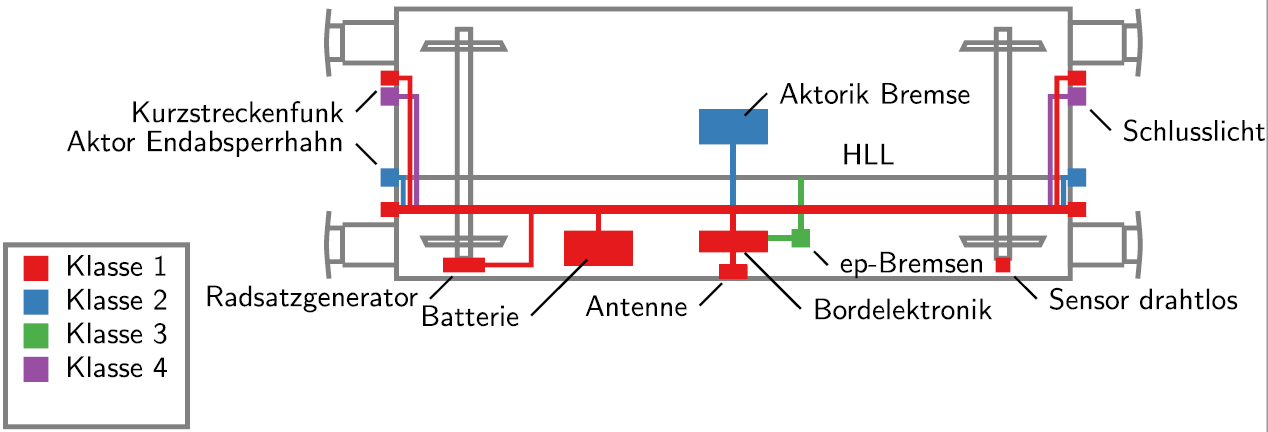
\includegraphics[width=\textwidth]{Bilder/Ausbaustufen_4.PNG}
    \caption{Klasse 4 bestehend aus Klasse 3 und der Automatisierung des Zugschlusses - angelehnt an \cite{Ausbaustufen}}
    \label{fig:Klasse4}
\end{figure} 
In der vierten Ausbaustufe ist ein automatisierter Zugschluss geplant, neben der dann noch lästigen Aufgabe den kompletten Wagenzug langzulaufen um am letzen Wagen ein Zugschluss-Signal zu stecken soll mit dieser Funktion auch die Zugintigrität gewährleistet werden.\par
\textbf{Ausbaustufe 5: Ausbaustufe 4 + Rangierantrieb}\par
\begin{figure}[htbp] 
    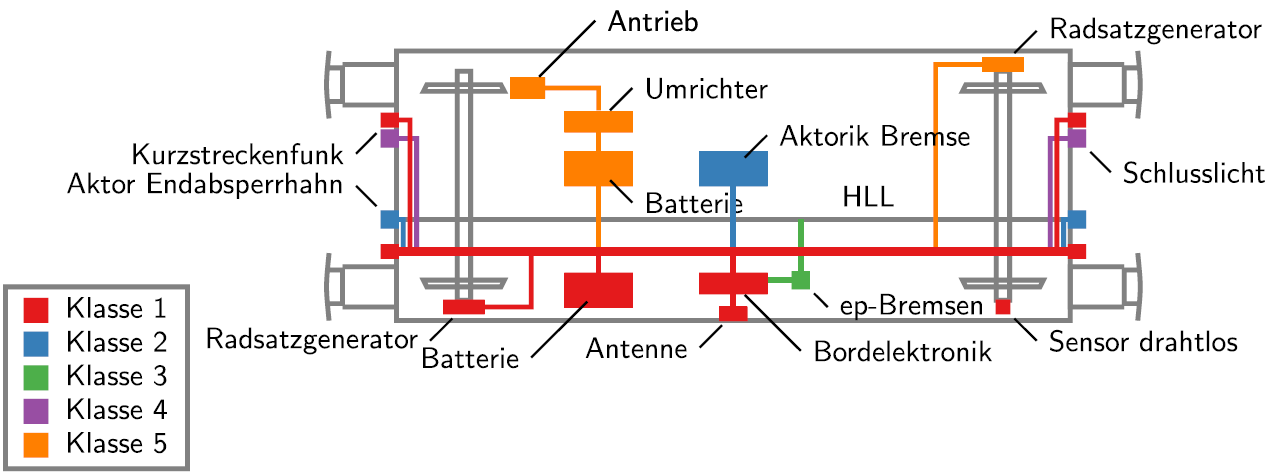
\includegraphics[width=\textwidth]{Bilder/Ausbaustufen_5.PNG}
    \caption{Klasse 5 bestehend aus Klasse 4 und einem Rangierantrieb - angelehnt an \cite{Ausbaustufen}}
    \label{fig:Klasse5}
\end{figure} 
In der fünften Ausbaustufe kommt der Rangierantrieb hinzu. Damit dieser ohne Probleme funktioniert brauch er er zusätzlich eine weitere Batterie und Umrichter. Zur Speisung der zweiten Batterie wird auch ein zweiter Radsatzgenerator eingebaut.\par
In diesem Stadium kann von einem automatisierten Güterwagen gesprochen werden. Er kann selbstständig bei der Briefkastenbedienung assistieren und auf dem Werksgelände ohne Rangierlok verfahren.\par
Die ersten drei Ausbaustufen sollen in diesem Projekt stattfinden. Ausbaustufe 4 und 5 in Folgeprojekten. Eine Zulassung soll über mindestens gleichbleibende Sicherheit bei kompletter Abschaltung des Systems stattfinden. Diese in Schritten stattfindende Automatisierung führt zu einem hohen Mehrwert des Güterwagens, nicht nur, im Einzelwagenverkehr.
 %\newpage
%\section{Anforderungen}
\textbf{Einfügen: Wie lang sind Lösezeiten, Verwendung Handbremse, Umlegen Endabsperrhähne}\par
\textbf{Sicherheitsrelevanz, Bedienen, Beobachten, Anbringungspunkte von Bauteilen -- gefedert? -- Bahntauglichkeit}\par
\subsection{Allgemeine und nicht funktionale Anforderungen}














%\begin{feat}
%automatische Zugschlussanzeige
%\end{feat}
%\begin{feat}
%Rangierantrieb
%\end{feat}%\newpage
%\section{Fazit} %\newpage

%Verzeichnisse
\listoffigures \addcontentsline{toc}{section}{Abbildungsverzeichnis}
\printbibliography[heading=bibintoc, title={Quellenverzeichnis}]

\newpage
%Anhang
\appendix
\section{Bremsprobe}\newpage
\section{RIL 936 - Technische Wagenbehandlung im Betrieb (Güterwagen) - Auszug}
Die Technischen Wagenbehandlungsarten stellen sicher,
dass die im Einsatz befindlichen Wagen betriebssicher
sind. Die Prüfung der Verkehrstauglichkeit ist besonders
geregelt.\par 
Die technische Wagenbehandlung darf nur durchgeführt
werden, wenn die Bedingungen des Arbeitsschutzes hergestellt
sind.\par
Die technischen Wagenbehandlungsarten werden in folgenden
Stufen ihrer Ausführung beschrieben.
\subsection{TWb Stufe 1: Behandlung vor einer Rangierfahrt}
\textbf{Ziel}\par
Durch die Behandlung der Stufe 1 soll der betriebssichere
Zustand der Wagen sowie deren Ladungen und intermodale
Ladeeinheiten (ILE) für die anschließende Rangierfahrt
festgestellt werden.\par
\textbf{Arbeitsumfang}\par
Die Behandlung der Stufe 1 beinhaltet eine Sichtprüfung
der Wagen, Ladungen und ILE auf Schäden und Mängel,
welche die Sicherheit der Rangierfahrt beeinträchtigen –
soweit sie vom Boden aus, neben dem Fahrzeug stehend,
erkennbar sind.\par
Dabei werden Wagen, Ladungen oder ILE nicht betreten
oder geöffnet.\par
Wagen, Ladungen und ILE werden in der Behandlungsstufe
1 augenscheinlich daraufhin geprüft, ob z.B.
\begin{itemize}
    \item die ordnungsgemäße Stellung von Türen, Schiebewände, Hauben, Dächer, Klappen, Sicherungsmittel usw. geschlossen und verriegelt sind, offensichtliche Schäden vorliegen, z. B. durch die Be- oder Entladung bzw.
    \item Eingriffe oder Manipulationen vorliegen,
    \item Tritte, Griffe, Handläufe und Aufstiegsleitern in bestimmungsgemäßem Zustand sind,
    \item kein Ladegut austritt,
    \item lose Wagenbestandteile ordnungsgemäß festgelegt oder befestigt sind,
    \item keine losen Gegenstände auf dem Wagen liegen, die die Betriebssicherheit gefährden können und
    \item Ladungssicherungen nicht beschädigt sind.
\end{itemize}
\textbf{Einzuleitende Maßnahmen und Dokumentation}\par
Bei erkannten Schäden und Mängeln sind Maßnahmen wie
\begin{itemize}
    \item Schaden oder Mangel selbst beheben (z.B. Tür schließen).
    \item Wagen von der Rangierfahrt ausschließen
\end{itemize}
einzuleiten.\par
Können vorgefundene Schäden/ Mängel nicht behoben
werden, sind erforderliche Maßnahmen über die zuständige
Dispostelle einzuleiten.
\subsection{TWb Stufe 2: Prüfung nach Abstellung (PnA}
\textbf{Ziel}\par
Durch die Behandlung der Stufe 2 sollen Einwirkungen Dritter während der Abstellzeit des Zuges (Wagen, Ladungen und ILE) festgestellt bzw. behoben werden, um für die anschließende Zugfahrt (inkl. Feststellen der Fahrbereitschaft) den sicheren Betrieb zu gewährleisten.\par
\textbf{Arbeitsumfang}\par
Die Behandlung Stufe 2 beinhaltet zur Feststellung der
Abfahrbereitschaft eine beidseitige Sichtprüfung der Wagen,
Ladungen und ILE. \par
Wagen, Ladungen und ILE werden augenscheinlich auf offensichtliche
Eingriffe oder Manipulationen geprüft.\par
Bei dieser augenscheinlichen Behandlung ist besonders
darauf zu achten, dass z.B.
\begin{itemize}
    \item Türen, Seitenwände, Dächer und Hauben usw. am Fahrzeug geschlossen und verriegelt sind,
    \item lose/bewegliche Fahrzeugteile festgelegt sind,
    \item Fahrzeuge ordnungsgemäß gekuppelt sind,
    \item Ladungssicherungen nicht beschädigt oder offensichtlich entfernt sind und
    \item dass kein Ladegut austritt.
\end{itemize}
Bei der Behandlung der Stufe 2 muss der Abgleich der ersten und letzten Wagennummer (Wagenliste oder Bremszettel) durchgeführt werden.\par
\textbf{Einzuleitende Maßnahmen und Dokumentation}\par
Bei erkannten Schäden und Mängel sind Abhilfemaßnahmen wie
\begin{itemize}
    \item Schaden oder Mangel selbst beheben (z.B. Tür schließen)
    \item Wagen von der Zugfahrt ausschließen einzuleiten.
\end{itemize}
Festgestellte Schäden und Mängeln sind mit Schadzettel (z.B. Störmeldezettel Tf) zu dokumentieren und dem zuständigen Disponenten zu melden. Können Sie deren Auswirkungen nicht sicher abschätzen oder nicht beheben, ist die weitere Vorgehensweise mit dem zuständigen Disponenten festzulegen.\par
Vor dem Einleiten von Abhilfemaßnahmen nach offensichtlichen Eingriffen oder von Manipulationen an Wagen wie z.B. geöffnete Türen/Verschlüsse oder das Anbringen
von nicht identifizierbaren Gegenständen, ist die weitere Vorgehensweise unverzüglich mit der zuständigen Dispostelle abzustimmen. Weitere Maßnahmen könnten von dem Ergebnis der Spurensicherung durch die Polizeibehörden abhängig sein. \par
Hinweise auf Schäden und Mängel sowie weiterführende Regelungen und Maßnahmen, sind im „Kriterienkatalog für Schäden und Mängel“ der Ril 936ff geregelt.\par
\subsection{TWb Stufe 3: Prüfung vor der Zugfahrt}
\textbf{Ziel} \par
Feststellung des betriebssicheren Zustands der Wagen,
Ladungen und ILE vor der Zugfahrt.\par
\textbf{Varianten} \par
Für die Stufe 3 können verschiedene Varianten erforderlich sein:
\begin{itemize}
    \item Behandlung vor der Zugfahrt - DBCDE Verkehr
    \item Behandlung vor der Zugfahrt – AVV Verkehr
\end{itemize}
\textbf{Besonderheiten} \par
Sendungen, an deren Transport besondere Bedingungen gestellt sind (z.B. außergewöhnliche Sendungen, Militärverkehr (MV) usw.) bedürfen einer vorherigen Wagensonderuntersuchung
(WSU) im Rahmen der Stufe 4 mit Abnahme. Die Dokumentation ist nach Ril 936.0301 vorzunehmen.\par
\textbf{Arbeitsumfang} \par
Die Durchführung der Stufe 3 erfolgt i.d.R. am fertig gebildeten Zug/ Zugteil. Dabei werden Systemdaten grundsätzlich mittels vorhandener mobiler DV überprüft und dokumentiert. Grundsätzlich ist die Durchführung der Stufe 3 mit der Reihung zu verbinden.\par
Die Stufe 3 beinhaltet die Feststellung
\begin{itemize}
    \item des betriebssicheren Zustandes der Fahrzeuge und Ladungen,
    \item das Ladungen und deren Sicherung soweit einsehbar, nicht beschädigt sind,
    \item auf Überladung,
    \item der Einhaltung bestimmter Zugbildungskriterien wie z.B.
    \begin{itemize}
        \item Kuppelzustand allgemein (gekuppelt und geschlaucht),
        \item Prüfung auf das Einstellen nicht zugelassener Wagen (z.B. schwerbeschädigte Wagen),
        \item Prüfung auf außergewöhnliche Sendungen (Stellung im Zug, Schutzabstände),
        \item Prüfung der Schutzabstände bei Gefahrgutsendungen GGVSEB,
        \item Abgleich der Ladungsgewichte sowie Wagenreihungskontrolle.
    \end{itemize}
\end{itemize}
\textbf{Einzuleitende Maßnahmen und Dokumentation} \par
Bei erkannten Schäden und Mängeln sind Abhilfemaßnahmen wie
\begin{itemize}
    \item Schaden oder Mangel selbst beheben (z.B. Tür schließen),
    \item Wagen von der Zugfahrt ausschließen
\end{itemize}
einzuleiten.\par
Festgestellte Schäden und Mängel sind mit dem erforderlichen Schadzettel zu bezetteln, zu dokumentieren und soweit erforderlich dem zuständigen Disponenten zu melden. Können Sie deren Auswirkungen nicht sicher abschätzen oder nicht beheben, ist die weitere Vorgehensweise mit dem zuständigen Disponenten festzulegen.\par
Hinweise auf Schäden und Mängel sowie weiterführende Regelungen und Maßnahmen, sind im „Kriterienkatalog für Schäden und Mängel“ der Ril 936ff geregelt.
\subsection{TWb Stufe 4: Untersuchung und Qualitätscheck Wagen}
\textbf{Ziel} \par
Die Feststellung des betriebssicheren Zustands der Wagen,
Ladungen und ILE.
\begin{itemize}
    \item Beurteilung von Schäden und Mängel und ausführliche Dokumentation,
    \item Prüfung auf uneingeschränkte Nutzbarkeit bzw. Festlegung der weiteren Einsatzkriterien und ausführliche Dokumentation
    \item Abhilfe durch Kleinstschadenbeseitigung oder Behandlung zum Verbleib im Betrieb.
    \item Erfassung und Beschreibung von Schäden zur Arbeitsvorbereitung für die Instandhaltung und Entscheidungsfindung für den Halter.
\end{itemize}
\textbf{Varianten} \par
Für die Stufe 4 können verschiedene Untersuchungen erforderlich sein:
\begin{itemize}
    \item Untersuchung von Wagen am Zug oder Zugteil
    \item Untersuchung von leeren Wagen vor der Beladung am Zug oder Zugteil im kombinierten Verkehr (siehe Ril 936.0103 KV)
    \item Untersuchung von beladenen Wagen am Zug oder Zugteil im Militärverkehr (siehe Ril 936.0104 MV)
\end{itemize}
Für die Durchführung der WSU ist, soweit diese Tätigkeiten nicht im Zeitfenster der Behandlungsart durchgeführt werden können, eine besondere Beauftragung nach Ril 936.0301 (Vordruck 936.0301V32) erforderlich.\par
\textbf{Besonderheiten} \par
Wird eine Untersuchung der Stufe 4 durchgeführt, ersetzt diese die Stufe 1, 2, 3, 3 KV und 3 AVV in jedem Fall. \par
\textbf{Arbeitsumfang} \par
Die Durchführung der Stufe 4 erfolgt i.d.R.am fertig gebildeten Zug/ Zugteil. Dabei werden Systemdaten grundsätzlich mittels vorhandener mobiler DV überprüft und dokumentiert. Grundsätzlich ist die Durchführung der Stufe 4 mit der Reihung zu verbinden. Weiter sind erforderliche Beschädigungs- und Mängelberichte zu erstellen.\par
Die Stufe 4 beinhaltet die Feststellung
\begin{itemize}
    \item des betriebssicheren Zustandes der Fahrzeuge und Ladungen,
    \item das Ladungen und deren Sicherung soweit einsehbar, nicht beschädigt sind,
    \item auf Überladung
    \item bestimmter Zugbildungskriterien wie z.B.
    \begin{itemize}
        \item Kuppelzustand allgemein (gekuppelt und geschlaucht),
        \item Prüfung auf das Einstellen nicht zugelassener Wagen (z.B. schwerbeschädigte Wagen),
        \item Prüfung auf außergewöhnliche Sendungen (Stellung im Zug, Schutzabstände),
        \item Prüfung der Schutzabstände bei Gefahrgutsendungen GGVSEB,
        \item Abgleich der Ladungsgewichte sowie Wagenreihungskontrolle.
    \end{itemize}
\end{itemize}
Die Suche nach verdeckten oder schwer erkennbaren Schäden und Mängeln muss erfolgen, wenn Merkmale an den Bauteilen, die Lage der Bauteile zueinander, Funktionsstörungen oder andere Gründe auf das Vorliegen von Unregelmäßigkeiten schließen lassen. Das dabei erforderliche Messen und Berechnen einzelner Maße ist unter Verwendung von Hilfs- und Messmitteln durchzuführen.\par
\textbf{Einzuleitende Maßnahmen und Dokumentation} \par
Bei erkannten Schäden und Mängeln sind Abhilfemaßnahmen wie
\begin{itemize}
    \item Schaden oder Mangel selbst beheben (siehe Ril 936.13 bzw. 936.95),
    \item Wagen von der Zugfahrt ausschließen
\end{itemize}
einzuleiten.




\end{document}